\documentclass[a4paper,14pt]{extarticle}

\usepackage[a4paper,top=20mm,bottom=20mm,left=30mm,right=10mm]{geometry}
\usepackage[T1,T2A]{fontenc}
\usepackage[utf8]{inputenc}
\usepackage[russian]{babel}
\usepackage{indentfirst}
\usepackage{titlesec}
\usepackage{graphicx}
\usepackage{listings}

\renewcommand{\baselinestretch}{1.3}
\titleformat{\section}{\normalsize\bfseries}{\thesection}{1em}{}
\titleformat{\subsection}{\normalsize\bfseries}{\thesection}{1em}{}
\setlength{\parindent}{12.5mm}

\begin{document}
	
	\newpage\thispagestyle{empty}
	\begin{center}
		\MakeUppercase{
			Министерство науки и высшего образования Российской Федерации\\
			Федеральное государственное бюджетное образовательное учреждение высшего образования\\
			<<Вятский Государственный Университет>>\\
		}
		Институт математики и информационных систем\\
		Факультет автоматики и вычислительной техники\\
		Кафедра электронных вычислительных машин
	\end{center}
	\vfill
	
	\begin{center}
		Отчет по лабораторной работе №6\\
		по дисциплине\\
		<<Информатика>>\\
		<<Кодирование информации>>
	\end{center}
	\vfill
	
	\noindent
	\begin{tabular}{ll}
		Выполнил студент гр. ИВТб-1301-05-00 \hspace{5mm} &
		\rule[-1mm]{25mm}{0.10mm}\,/Макаров С.А./\\
		
		Руководитель доцент кафедры ЭВМ & \rule[-1mm]{25mm}{0.10mm}\,/Коржавина А.С./\\
	\end{tabular}
	
	\vfill
	\begin{center}
		Киров 2024
	\end{center}
	
	\newpage
	\section*{Цель}
	Цель лабораторной работы: закрепить на практике знания форматах представления числовой информации. Написать программы, решающие описанные ниже задачи.
	
	\section*{Задание}
	\begin{enumerate}
		\item Равномерное кодирование. Написать программу, выполняющую кодирование N различных состояний равномерно. На входе: целое число N -- количество различных состояний, на выходе -- список кодов.
		
		\item Оптимальное кодирование. Написать программу, выполняющую кодирование алгоритмом Хаффмана или Фано. На входе через пробел: количество событий (кодовых состояний), массив вероятностей каждого из событий. На выходе: коды состояний.
	\end{enumerate}
	
	\newpage
	\section*{Решение}
	\subsection*{Задание 1}
	Схема алгоритма для решения предлагаемой задачи представлена на рисунке 1.
	\begin{figure}[h]
		\centering
		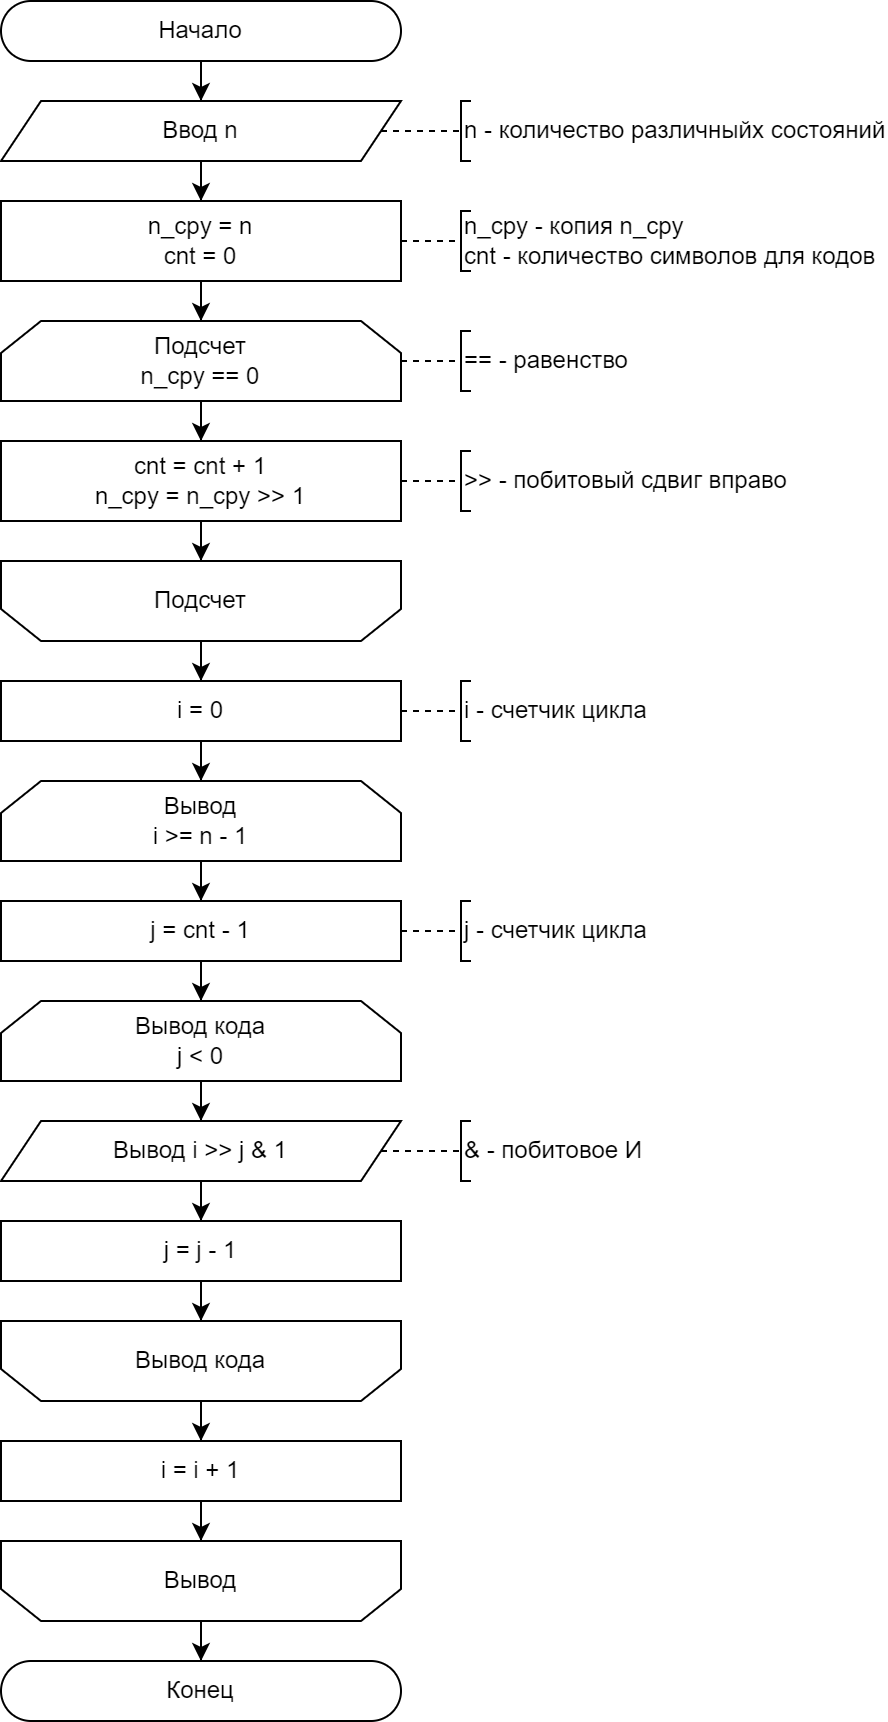
\includegraphics[width=0.6\linewidth]{schemes/s-1}
	\end{figure}
	\begin{center}
		Рисунок 1 – Схема алгоритма задания 1
	\end{center}
	
	\pagebreak
	\begin{lstlisting}[tabsize=2,basicstyle=\ttfamily]
#include <stdio.h>
int main() {
	int n;
	scanf("%d", &n);
	int n_cpy = n, cnt = 0;
	while (n_cpy) cnt++, n_cpy >>= 1;
	for (int i = 0; i < n; i++) {
		for (int j = cnt - 1; j >= 0; j--) {
			printf("%d", i >> j & 1);
		}
		printf(" ");
	}
	return 0;
}
	\end{lstlisting}
	
	\newpage
	\subsection*{Задание 2}

	\section*{Вывод}
	
\end{document}